\lesson{1}{2023-10-16 20:17}{Vectors}
\chapter{Vectors}

\section{Introduction}

\begin{definition}[Vectors]
  Vectors are mathematical objects with both {\bf magnitude} and {\bf direction}.
\end{definition}
Geometrially, vectors can be thought of as arrows/direced line segments in space in space.
\begin{figure}[H]
\centering
   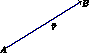
\includegraphics[scale=3.0]{vector.pdf}
   \caption{A Vector}
   \label{fig:figure-1-vector}
\end{figure}


\begin{eg}[Examples of vectors]
  Here are some important examples of vectors\\
  \vspace{-10px}
  \begin{itemize}
    \item The displacement of a particle is a vector.
    \item The velocity of a particle is a vector.
    \item The force acting on a particle is a vector.
  \end{itemize}

\end{eg}

\begin{notation}
  Vectors can be denoted in 3 ways,
  \begin{itemize}
    \item Using {\bf boldface notation}: $\boldsymbol{V}$
    \item Underlining:  $\underline{V}$ 
    \item An arrow over the symbol: $\vec{V}$

  \end{itemize}


\end{notation}

\section{Euclidean Three Space $\mathbb{E}^3$}

\begin{definition}[Euclidian Three Space]
 
  Euclidean Three Space is the set of all ordered triples of real numbers.\\
  \vspace{-10px}
  \begin{equation}
    \mathbb{E}^3 = \{(x,y,z) | x,y,z \in \mathbb{R}\}
  \end{equation}

\end{definition}

The \textbf{axes} of $\mathbb{E}^{3}$ are the $x$, $y$ and $z$, i.e.
\vspace{-10px}
\begin{equation}
  x = (x,0,0), y = (0,y,0), z = (0,0,z)
\end{equation}

We orient the axis according to the \textbf{right hand rule}. This is shown in the following diagram:

%generate tikz code for axes in 3d space

\begin{figure}[H]
  \centering
  \begin{tikzpicture}
    \draw[->] (0,0,0) -- (3,0,0) node[anchor=north east]{$y$};
    \draw[->] (0,0,0) -- (0,3,0) node[anchor=north west]{$z$};
    \draw[->] (0,0,0) -- (0,0,3) node[anchor=south]{$x$};
  \end{tikzpicture}
  \caption{Axes in $\mathbb{E}^3$}
\end{figure}

\begin{note}
  We need to pick an \textbf{origin} and stay with it. We will use the origin $(0,0,0)$.
\end{note} 

\section{Vectors in $\mathbb{E}^3$}
\subsection{Distance in $\mathbb{E}^3$}
Let $P$ and $P^{'}$ be points in $\mathbb{E}^3$. And let $P = (x,y,z)$ and $P^{'} = (x^{'},y^{'},z^{'})$.
\begin{definition}[Distance in $\mathbb{E}^3$]
  The \textbf{distance} between $P$ and $P^{'}$ is defined as:
  \begin{equation}
    d(P,P^{'}) = \sqrt{(x-x^{'})^2 + (y-y^{'})^2 + (z-z^{'})^2}
  \end{equation}
\end{definition}
This is illustrated in the following diagram
\begin{figure}[H]
\centering
   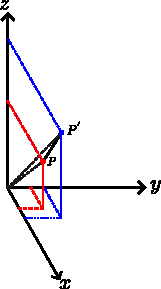
\includegraphics[scale=1.75]{distance.pdf}
   \caption{Distance in $\mathbb{E}^3$}
   \label{fig:figure-8-space}
\end{figure}
\clearpage
\subsection{Vectors in $\mathbb{E}^3$}
\begin{definition}[Vectors in $\mathbb{E}^3$]
  A \textbf{vector} in $\mathbb{E}^3$ is an ordered triple of real numbers.\\
  \vspace{-10px}
  \begin{equation}
    \vec{v} = (v_1,v_2,v_3)
  \end{equation}
\end{definition}

\begin{Notation}
  We can also represent vectors using {\bf column notation}
  $$\underline{v} = \begin{bmatrix} v_1 \\ v_2 \\ v_3\end{bmatrix} $$
  
\end{Notation}

